\chapter{Higgs boson reconstruction in the higgsino search}
\label{app:higgs}

This appendix discusses the approaches that have been tested for the reconstruction of the 
candidate Higgs bosons for the higgsino search described in Chapter \ref{chap:ewk_prod}. 
The signal events considered in this appendix are those where both Higgs bosons decay to a $b\bar{b}$ pair. 
As already discussed in Section \ref{sec:ewk:sigbkg}, the four jets selected to reconstruct the two Higgs bosons 
are selected with the following criteria:

\begin{itemize}
\item If there are exactly four $b$-tagged jets in the event, those are used.
\item If there are more than four $b$-tagged jets, the selected ones are the four $b$-tagged jets with highest \pt.
\item If there are less than four $b$-tagged jets, the selected ones are the $b$-tagged jets and the non-tagged jets with highest \pt.
\end{itemize}

Figure  \ref{fig:h_reco_match_possible}  shows the fraction of signal events that have four reconstructed jets, the fraction 
of signal events where it is possible to select the four correct jets originating from the decay of the Higgs bosons 
(which corresponds to requiring four jets with \pt $>$25 GeV  matched in dR$<$0.3 with the 4 $b$-quarks coming from the two Higgs bosons), 
and the fraction of signal events where the choice of jets described above selects the correct jets. 
The four jets selected are the correct set of jets about 70-80\% of the times that the correct match is possible. 


\begin{figure*}[h]
\centering
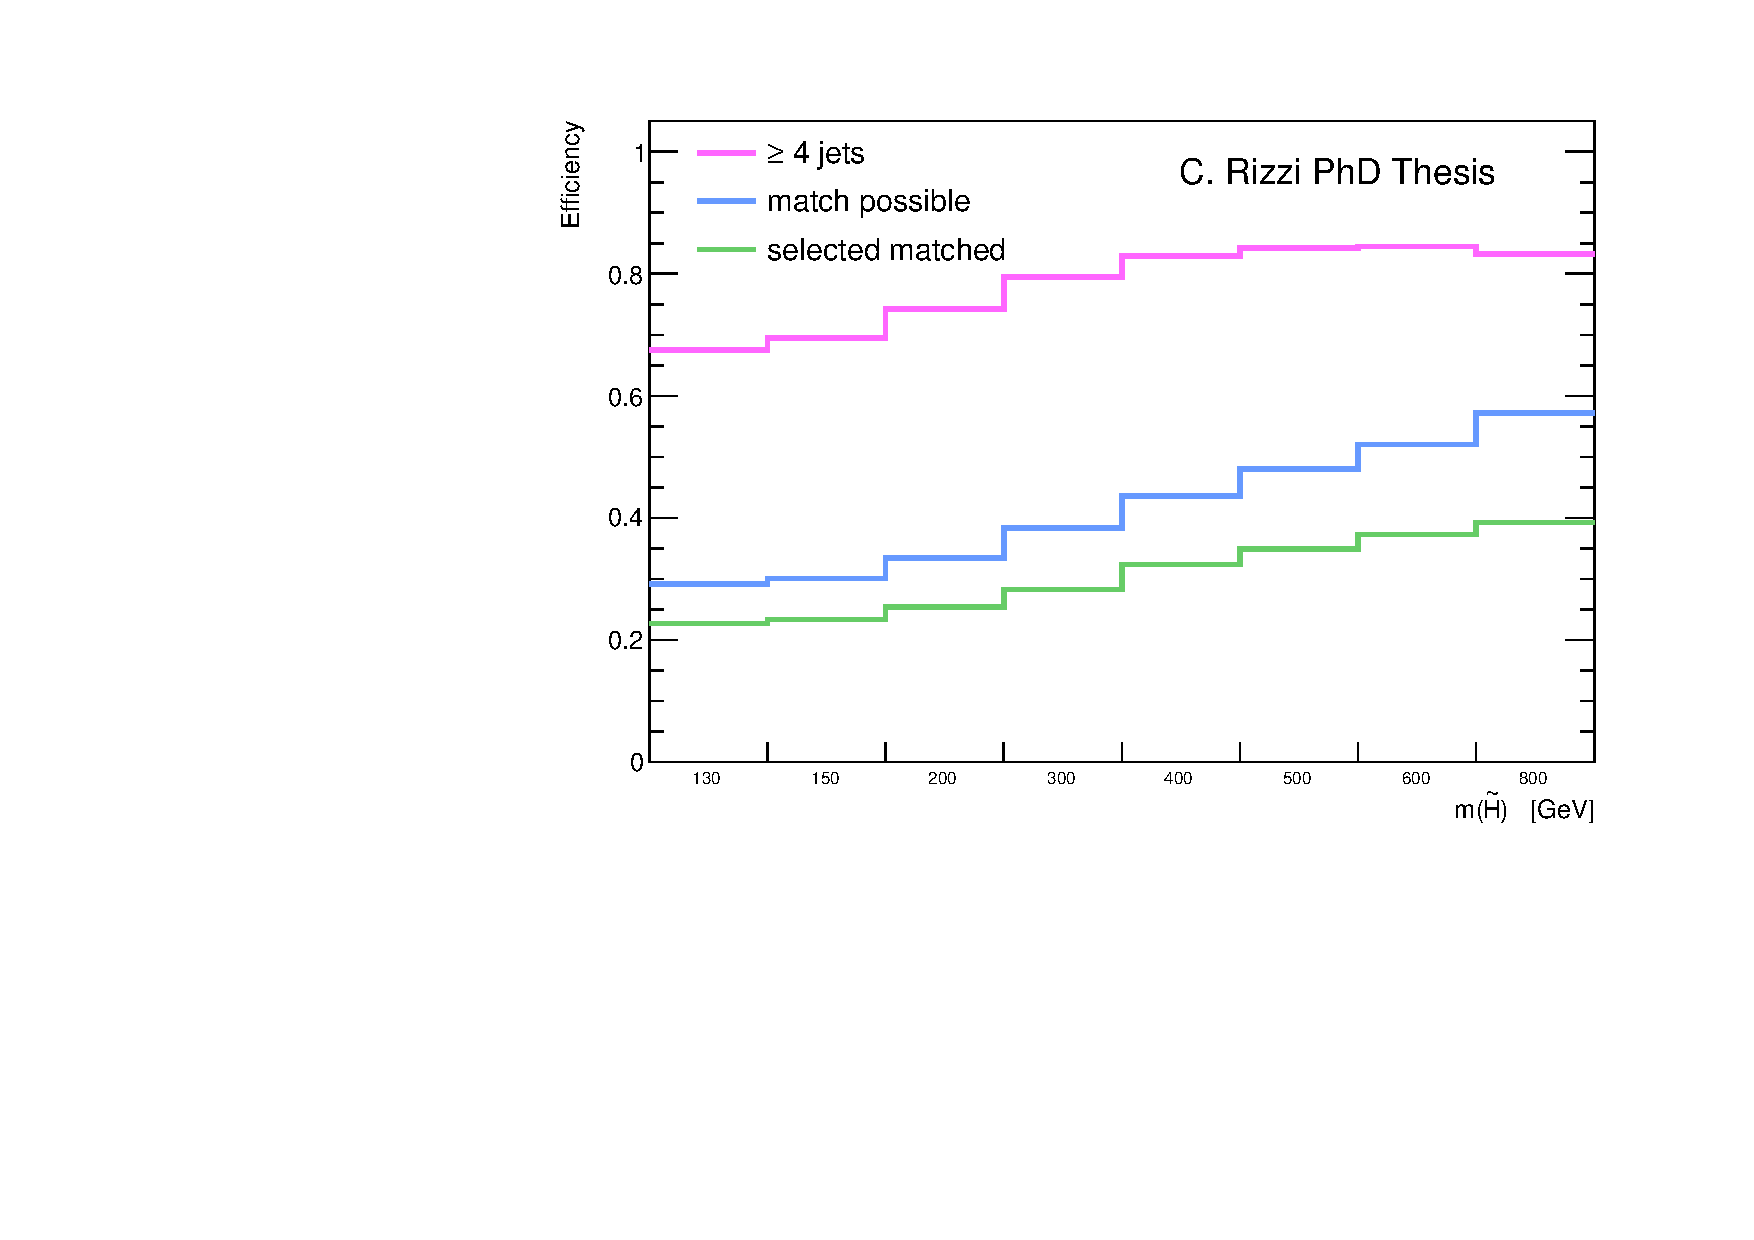
\includegraphics[width=0.7\textwidth]{figures/h_reco/match_possible.pdf}
\caption{Fraction of events where the algorithm described in the text selects the correct jets.}
\label{fig:h_reco_match_possible}
\end{figure*}

Once the four jets are selected, 
different algorithms to group them into pairs (each one corresponding to one of the two Higgs boson candidates) 
are compared: 

\begin{description}
%\item[115] Choose the pairing in which one of the masses is closer to 115 GeV (the value of 115 has been determined by signal studies showing that it was the peak of the reconstructed mass for the correct pairing).
\item[min-diff] Minimize the difference between m($h_1$)  and m($h_2$), where m($h_1$) and m($h_2$) are the masses of the two boson candidates and 
m($h_1$)$>$m($h_2$).
\item[min-dR] Minimize \dRmax (defined in Section \ref{sec:ewk:sigbkg}).
\item[max-\pt] Maximize min(\pt($h_1$), \pt($h_1$)).
\end{description}

%The performance of each of these algorithms has been compared, 
%taking as reference the number of times in which a correct reconstruction is  possible. 

Figure \ref{fig:h_reco_best_match} shows the fraction of times that each of the algorithms 
described above leads to the same pairs as the true matching, with respect to the number of events in which the true matching is possible. 
For signals with low higgsino mass the algorithm that minimize the mass difference performs better, 
while at high signal masses, where the two Higgs bosons (and their decay products) are more boosted, 
the min-dR algorithm reproduces the true matching a higher fraction of times. 
The max-\pt algorithm instead underperforms for all signal masses compared to the other 
two. 

\begin{figure*}[h]
\centering
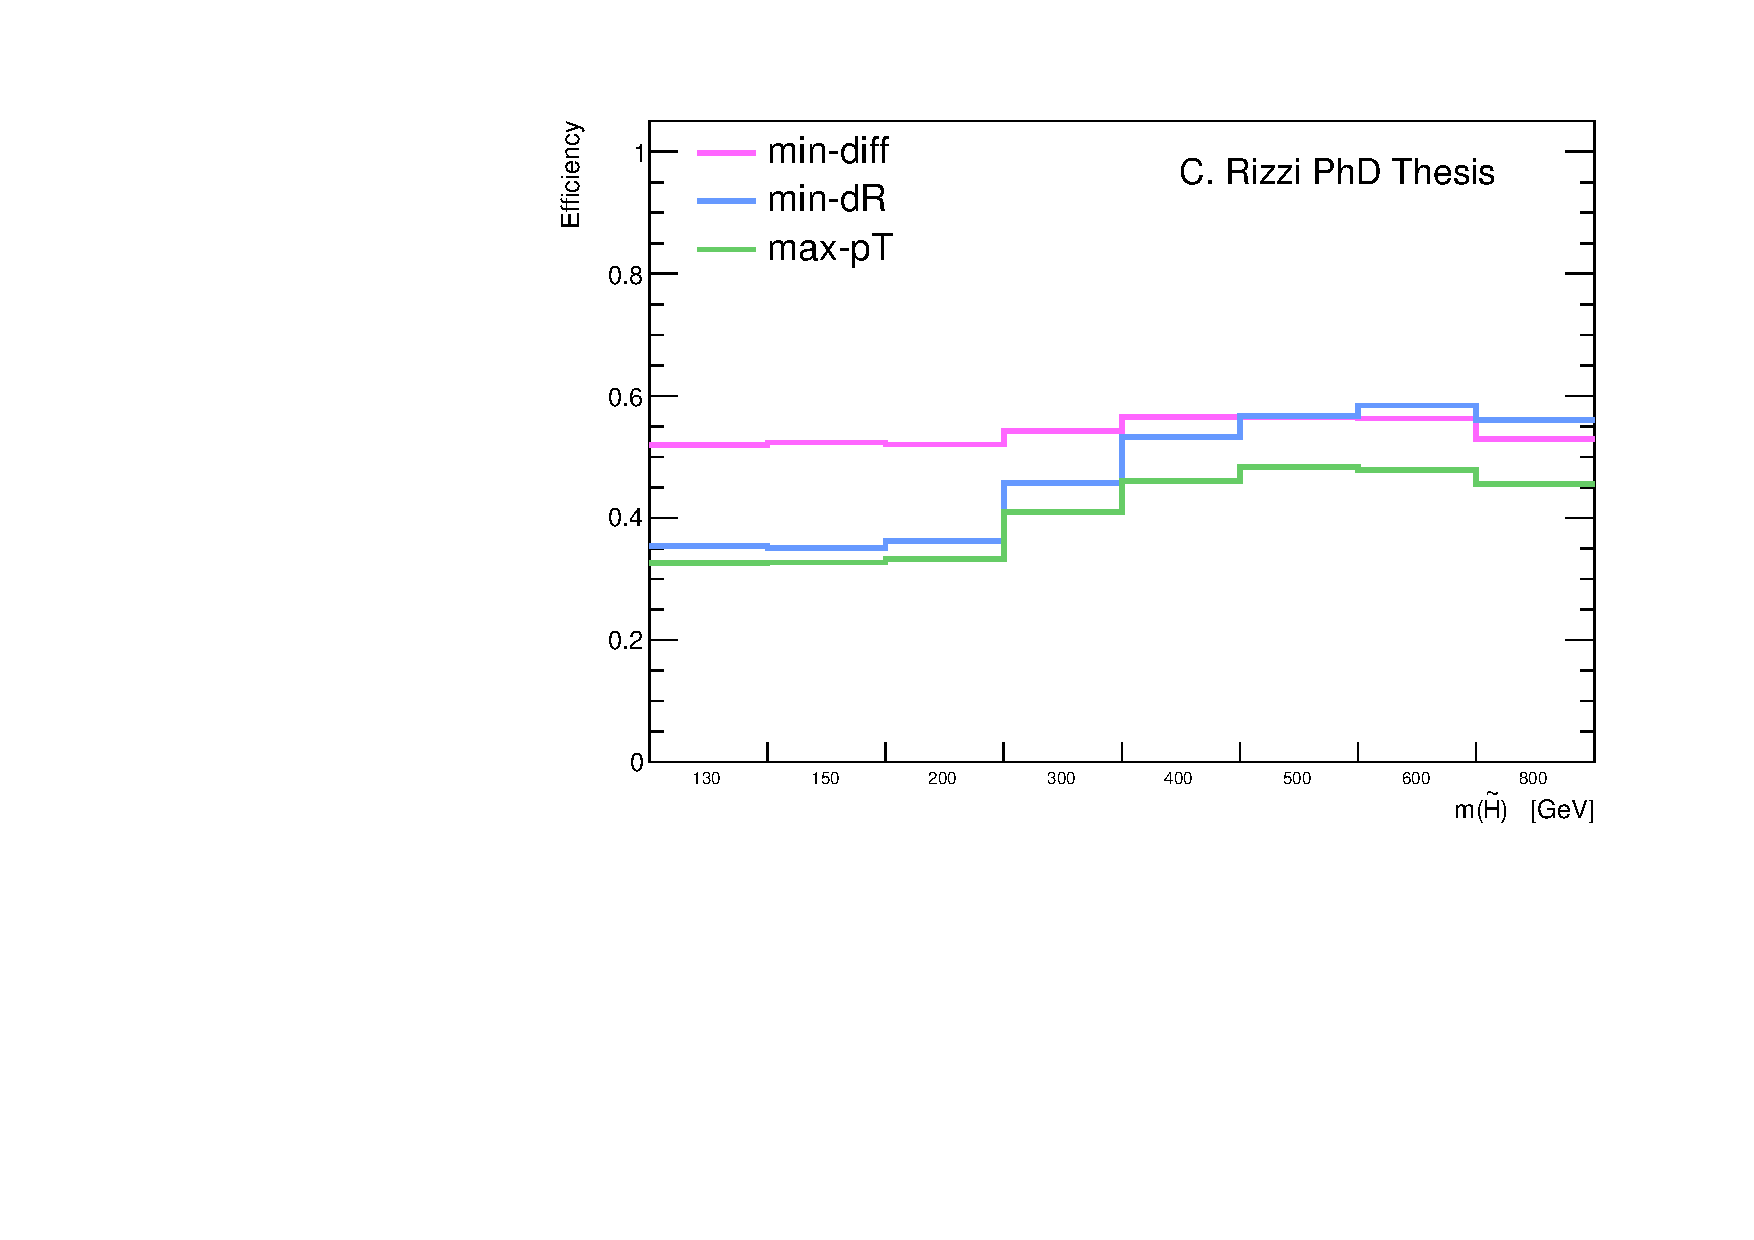
\includegraphics[width=0.7\textwidth]{figures/h_reco/best_match_if_match_possible.pdf}
\caption{Fraction of hh$\to$4b events where the reconstruction method indicated in the legend leads to the correct match. The fraction shown is with respect to the events where the correct match is possible.}
\label{fig:h_reco_best_match}
\end{figure*}

Figures \ref{fig:ewk:h1_mass} and \ref{fig:ewk:h2_mass} show the distribution of m($h_1$) and m($h_2$) 
respectively, for signal and background events normalized to unit area, 
with Higgs boson candidates reconstructed with the min-dR and min-diff algorithms. 
We can notice the different shape of the distributions with the two algorithms, especially in the case of m($h_2$). 
Considering that the high-mass analysis focuses on signals with intermediate and high higgsino mass, 
the min-dR algorithm was chosen as baseline algorithm for the reconstruction of the candidate Higgs bosons. 
This choice was confirmed by the optimization procedure described in Section \ref{sec:ewk:multibin}, 
where the values of the candidate Higgs bosons reconstructed with both algorithms have been used as input and 
the min-dR algorithm gave consistently better expected significances.  


\begin{figure*}[htbp]
\centering 
\subfigure[min-dR]{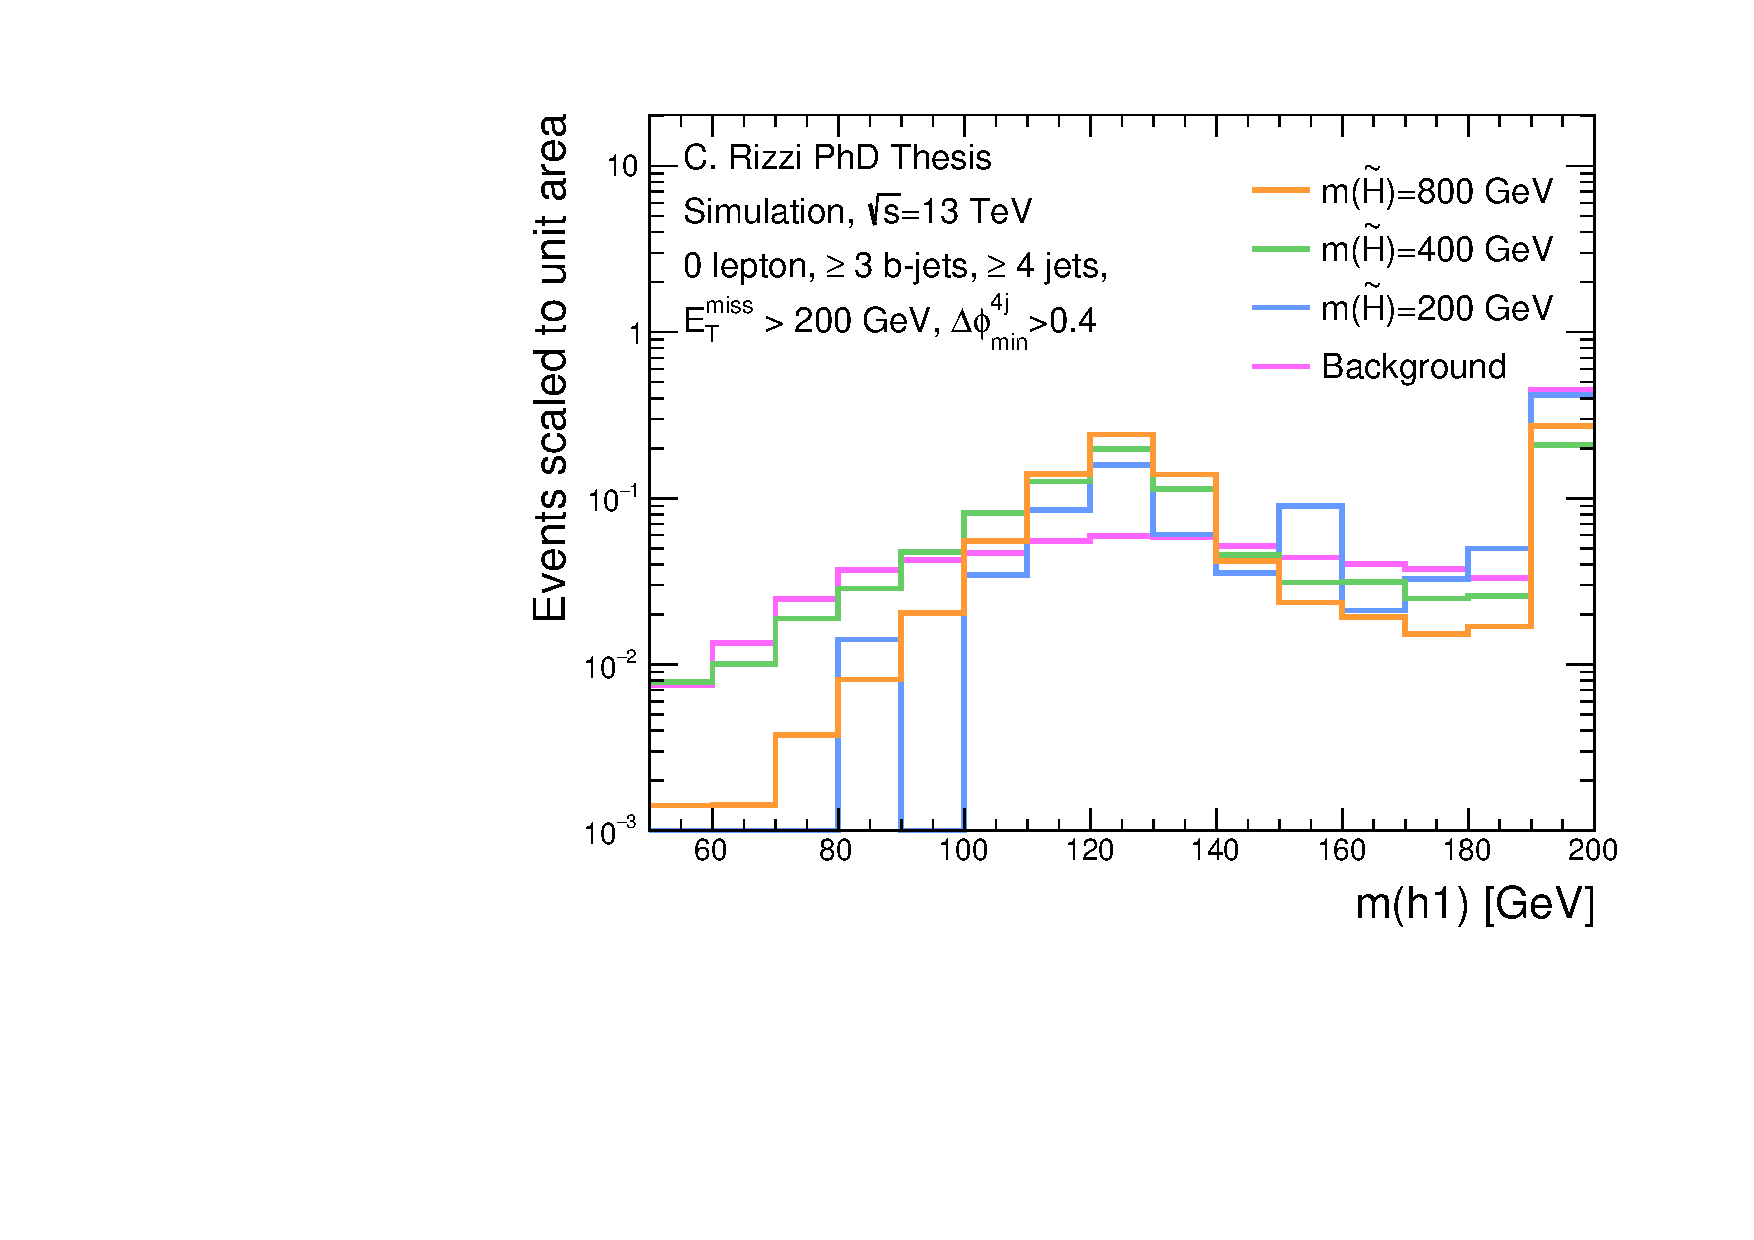
\includegraphics[width=0.48\textwidth]{figures/ewk_prod/h_mass/hh_compare_mass_h1_min_dR_scale.pdf}\label{fig:ewk:h_mass:mass_h1_min_dR}}
\subfigure[min-diff]{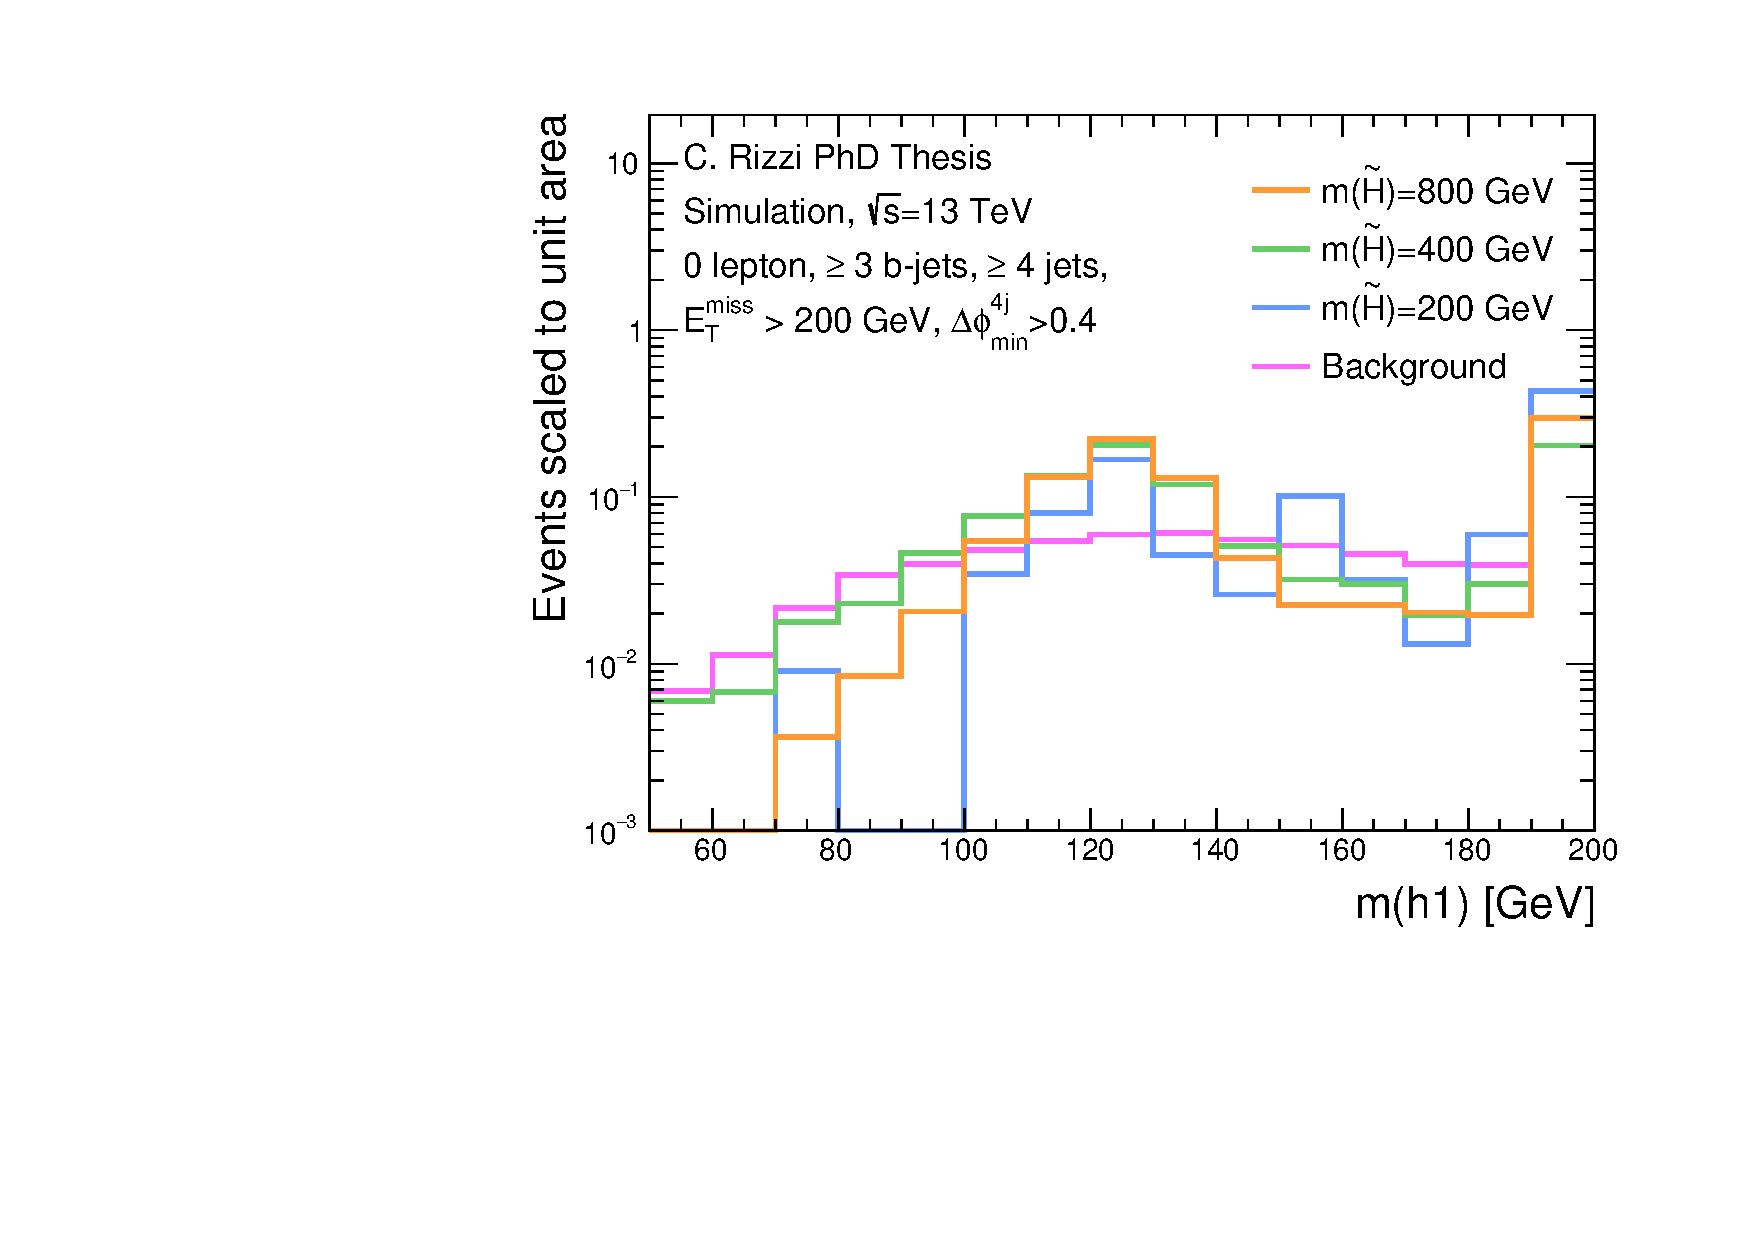
\includegraphics[width=0.48\textwidth]{figures/ewk_prod/h_mass/hh_compare_mass_h1_min_min_diff_scale.pdf}\label{fig:ewk:h_mass:mass_h1_min_diff}} 
\caption{Distribution of m($h_1$) in signal and background. The Higgs candidates are reconstructed with 
\subref{fig:ewk:h_mass:mass_h1_min_dR} the min-dR algorithm and 
\subref{fig:ewk:h_mass:mass_h1_min_dR} the min-diff algorithm. All distributions are normalized to unit area.}
\label{fig:ewk:h1_mass}
\end{figure*}

\begin{figure*}[htbp]
\centering 
\subfigure[min-dR]{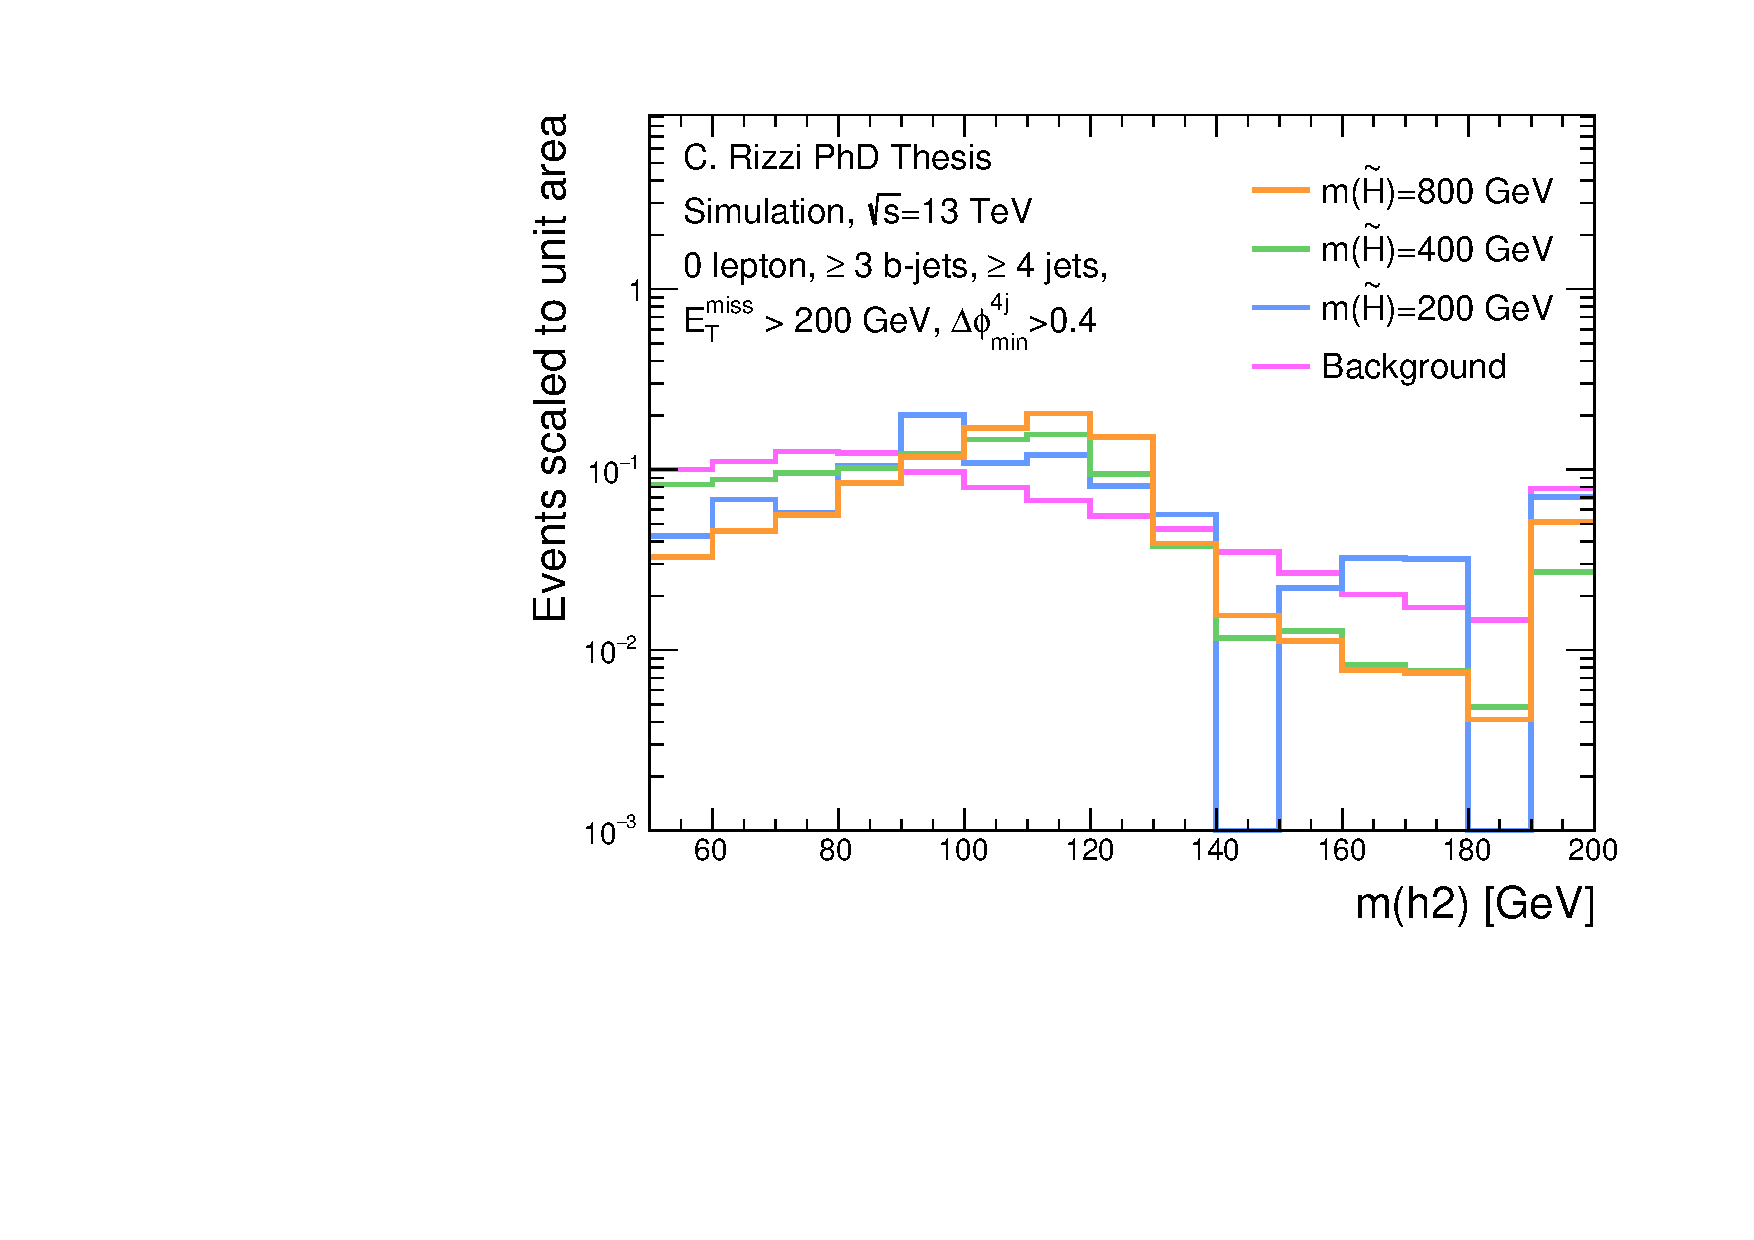
\includegraphics[width=0.48\textwidth]{figures/ewk_prod/h_mass/hh_compare_mass_h2_min_dR_scale.pdf}\label{fig:ewk:h_mass:mass_h2_min_dR}}
\subfigure[min-diff]{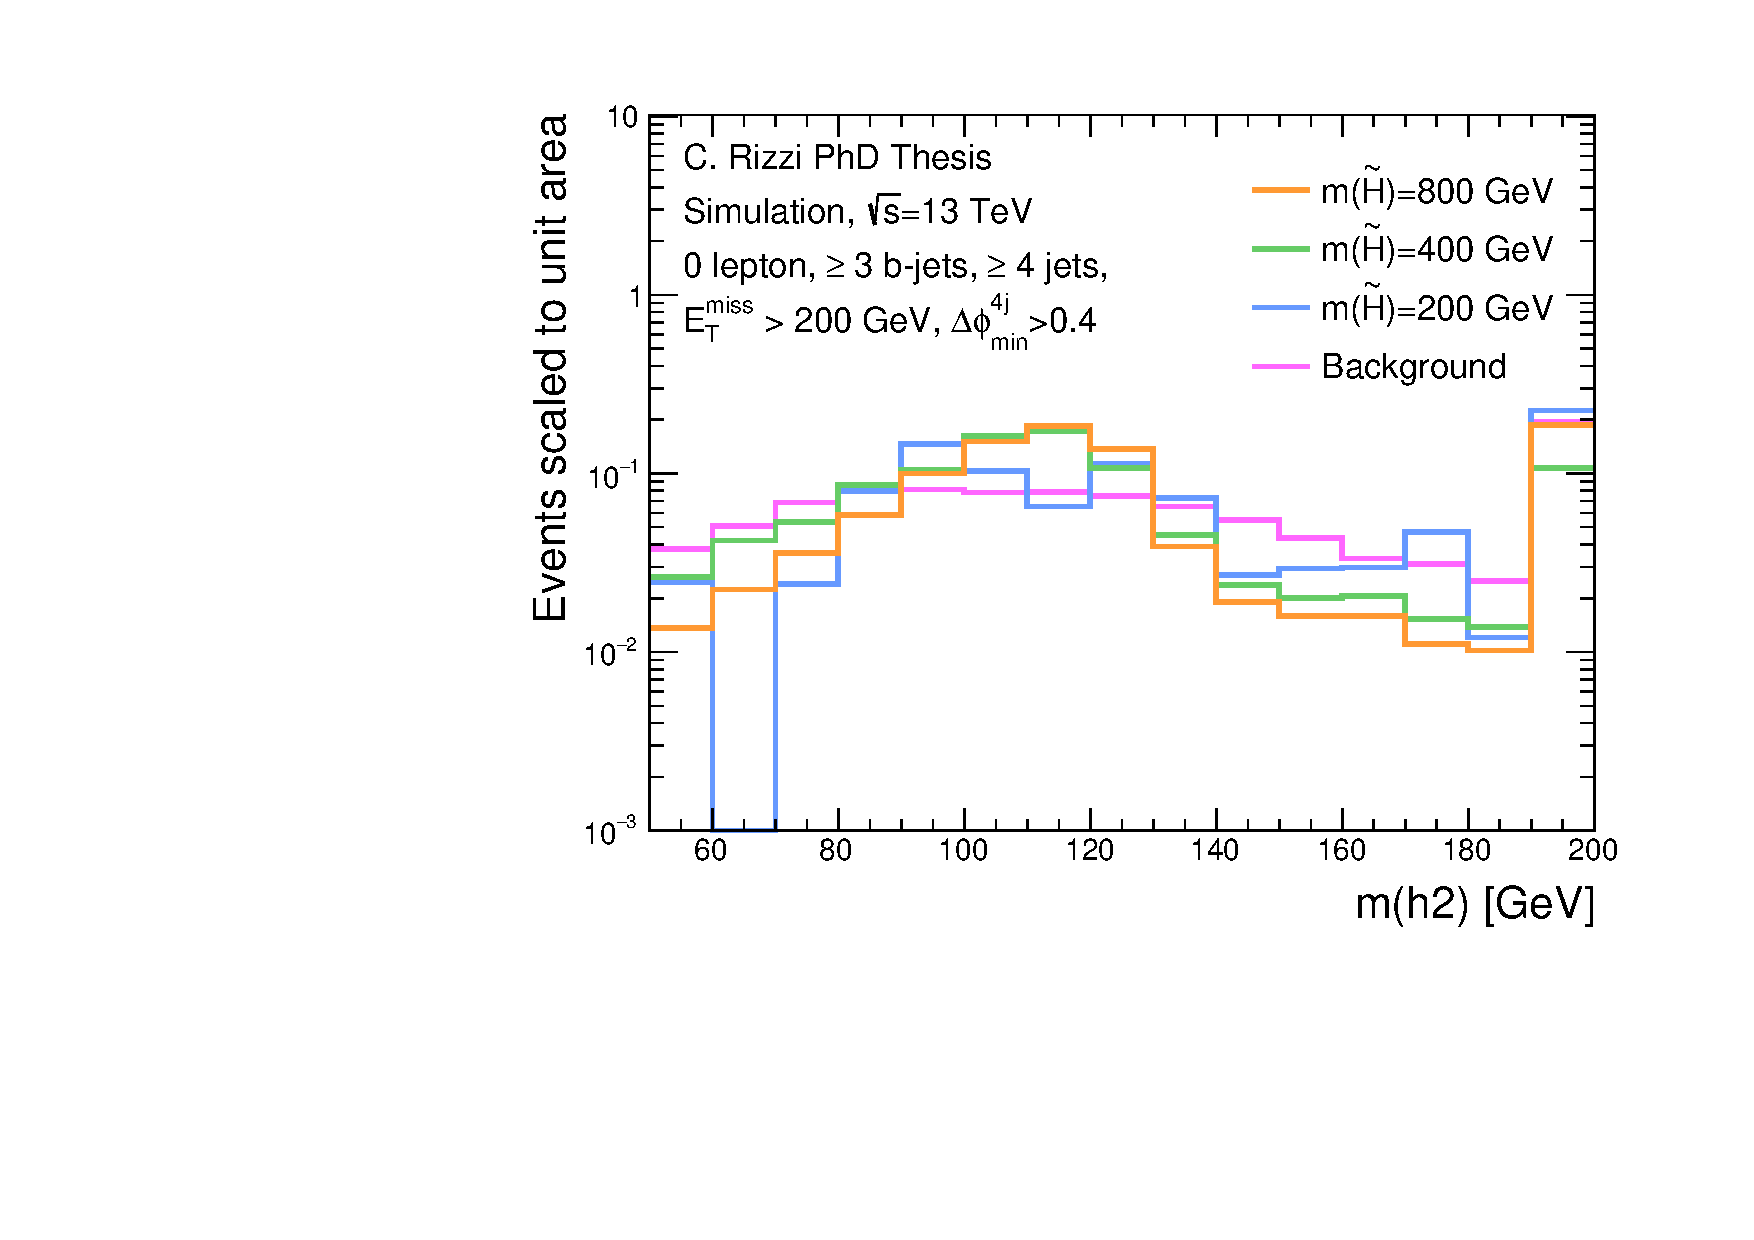
\includegraphics[width=0.48\textwidth]{figures/ewk_prod/h_mass/hh_compare_mass_h2_min_min_diff_scale.pdf}\label{fig:ewk:h_mass:mass_h2_min_diff}} 
\caption{Distribution of m($h_2$) in signal and background. The Higgs candidates are reconstructed with 
\subref{fig:ewk:h_mass:mass_h2_min_dR} the min-dR algorithm and 
\subref{fig:ewk:h_mass:mass_h2_min_dR} the min-diff algorithm. All distributions are normalized to unit area.}
\label{fig:ewk:h2_mass}
\end{figure*}
